\documentclass{article}

\usepackage{tikz}
\usetikzlibrary{calc}

%--------------------------------------------------
%: math3d
\tikzset{math3d/.style={x={(-0.353cm,-0.353cm)},z={(0cm,1cm)},y={(1cm,0cm)}}}

%--------------------------------------------------
\begin{document}

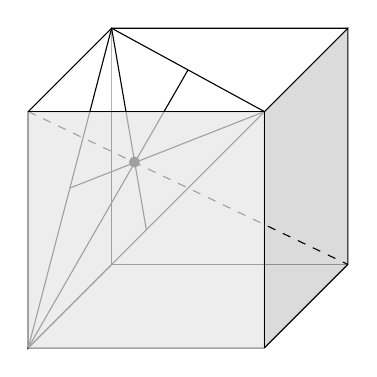
\begin{tikzpicture}[math3d, scale=3]
	% face inferieure ABCD, D=O
	\coordinate (a) at (1,0,0);
	\coordinate (b) at (1,1,0);
	\coordinate (c) at (0,1,0);
	\coordinate (d) at (0,0,0);
	% face superieure EFGH (obtenue par translation de ABCD)
	\coordinate (e) at (1,0,1);
	\coordinate (f) at (1,1,1);
	\coordinate (g) at (0,1,1);
	\coordinate (h) at (0,0,1);
	% les 3 aretes cachees, au fond, partant de O
	\draw (d) edge (a) edge (c) edge (h);
	\fill[fill=white, opacity=0.7] (e) -- (f) -- (g) -- (h) -- cycle; % dessus
	\fill[fill=gray!40, opacity=0.7] (b) -- (c) -- (g)-- (f) -- cycle; % droite
	\draw (a) -- (e) -- (f) -- (g) -- (c) -- (b) -- cycle; % 2 faces de devant
	\draw (e) -- (h) -- (g)  (b)--(f); % les aretes restantes
	% le centre de gravite
	\draw ($ 0.33*(a) + 0.33*(f) + 0.33*(h) $) node{$\bullet$};
	\draw[dashed] (e) -- (c);
	\draw (h) -- (f) -- (a) -- cycle;
	\draw (h) -- (1,1/2,1/2) ;
	\draw (a) -- (1/2,1/2,1) ;
	\draw (f) -- (1/2,0,1/2) ;
	\fill[fill=gray!20, opacity=0.7] (a) -- (b) -- (f) --(e) -- cycle; % avant
\end{tikzpicture}

\end{document}
